% !TEX root = mythesis.tex



%==============================================================================
\chapter{Theoretical concepts}
\label{sec:theory}
%==============================================================================

The purpose of this chapter is to provide a brief introduction to the underlying concepts and terminology used in particle physics. An overview of the Standard Model of particle physics is given, which describes the fundamental particles and the forces responsible for their interaction. Some drawbacks of the Standard Model are also discussed. Finally, a new exotic particle called vector-like quark is introduced.
%------------------------------------------------------------------------------
\section{Basic concepts}%
\label{sec:theory:basicconcepts}
%------------------------------------------------------------------------------

%------------------------------------------------------------------------------
\subsection*{Natural units}%
\label{sec:theory:basicconcepts:naturalunits}\index{basicconcepts}
%------------------------------------------------------------------------------
The S.I.\ units are comprised of [\si{\kilogram}, \si{\metre}, \si{\second}], which form a fundamental basis for the measurement of different macroscopic phenomena. However, it is not a common choice for the representation of the properties of sub-atomic particles. The system of units used in particle physics is known as \textit{natural units}. 

In natural units, \si{\planckbar} = \si{\clight} = 1 which means [$\si{\kilogram}$, $\si{\metre}$, $\si{\second}$] can be substituted by [$\si{\electronvolt}$, $\si{\electronvolt^{-1}}$, $\si{\electronvolt^{-1}}$], where $\si{\planckbar}$ is the reduced Planck's constant, $\si{\clight}$ is the speed of light in vacuum. For example, mass of a proton can be expressed as $\SI{1}{\giga\electronvolt}$.~\cite{thomson}


%------------------------------------------------------------------------------
\subsection*{Cross-section}%
\label{sec:theory:basicconcepts:crossection}\index{crossection}
%------------------------------------------------------------------------------
In particle physics, particle interactions such as scattering or decay processes are mainly concerned. Cross-section is a significant observable measured in the experiments. It is defined as the probability of occurrence of a given particle physics process. The cross-section of a given process is theoretically proportional to:

\begin{equation} \label{eqn:theory:basicconcepts:crossection}
	\sigma \propto \int {\lvert \mathcal{M} \rvert}^2 d\rho \,,
\end{equation}
where ${\lvert \mathcal{M} \rvert}^2$ is the square of the matrix element of the process. It is a measure of the transition amplitude from initial to the final state, and $\int d\rho$ is an integral over the phase space \cite{thesis:anji}. 

The cross-section has dimensions of area and is often expressed with \textit{barn} as its units where $\SI{1}{\barn} = \SI{1E-28}{\metre^2}$. The cross-sections for particle physics processes are typically at the higher energy scale, in the range of \textit{picobarn} (\si{\pico\barn}) to \textit{femtobarn} (\si{\femto\barn}), where \SI{1}{\pico\barn} = \SI{1E-12}{\barn} and \SI{1}{\femto\barn} = \SI{1E-15}{\barn} \cite{thomson}. 

%------------------------------------------------------------------------------
\subsection*{Luminosity}%
\label{sec:theory:basicconcepts:Luminosity}\index{Luminosity}
%------------------------------------------------------------------------------
The quantity that measures the ability of a particle accelerator to produce the required number of interactions is called the instantaneous luminosity $\mathcal{L}(t)$. It is defined as the proportionality factor between the number of events per second $\frac{dN}{dt}$ and the cross-section $\sigma$, given by Eqn.\ \ref{eqn:theory:basicconcepts:luminosity}

\begin{equation} \label{eqn:theory:basicconcepts:luminosity}
	\frac{dN}{dt} = \sigma \mathcal{L}(t) \,.
\end{equation} 
It has a dimension of events per time per area and is usually expressed in the units of $\si{\barn^{-1}}$. $\mathcal{L}(t)$ also depends on the particle beam parameters and the target properties. The integral of the instantaneous luminosity with respect to time is called the integrated luminosity $\mathcal{L}_{\text int}$, as shown below:
\begin{equation} \label{eqn:theory:basicconcepts:integratedluminosity}
\mathcal{L}_{\text int} = \int \mathcal{L}(t) \, dt \,.
\end{equation}
$\mathcal{L}_{\text int}$ is often used for characterising the performance of a particle accelerator. In particular, collider experiments aim to maximise their integrated luminosities. Higher integrated luminosity means more events available for analysis.~\cite{thomson}


%------------------------------------------------------------------------------
\subsection*{Decay width and Branching fraction}%
\label{sec:theory:basicconcepts:decaywidth}\index{decaywidth}
%------------------------------------------------------------------------------
The \textbf{Decay width $\Gamma$} is a physical observable measured in decay processes. It is inversely proportional to the lifetime $\tau$ of the original particle which decays into daughter particles and is expressed in units of $\si{\electronvolt^{-1}}$, given by Eqn.\ \ref{eqn:theory:basicconcepts:decaywidth}

\begin{equation} \label{eqn:theory:basicconcepts:decaywidth}
\Gamma = \frac{1}{\tau} \,.
\end{equation} 
Particles usually decay via different processes depending on the allowed interactions between mediator particles. If $\Gamma_{\text{i}}$ denotes the decay width of process i, then the total decay width $\Gamma_{\text{total}}$ can be written as: 

\begin{equation} \label{eqn:theory:basicconcepts:totaldecaywidth}
\Gamma_{\text{total}} = \sum_{i}^{}\Gamma_{\text{i}} \,.
\end{equation} 

\textbf{Branching ratio $\mathcal{B}_{\text{i}}$} of a given process can be defined as the ratio between the decay width $\Gamma_{\text{i}}$ and the total decay width. This can be expressed as:

\begin{equation} \label{eqn:theory:basicconcepts:branchingfraction}
\mathcal{B}_{\text{i}} = \frac{\Gamma_{\text{i}}}{\Gamma_{\text{total}}} \,.
\end{equation}


%------------------------------------------------------------------------------
\subsection*{Center-of-mass energy}%
\label{sec:theory:basicconcepts:centerofmass}\index{centerofmass}
Center-of-mass energy $\sqrt{s}$ is the total amount of energy available to produce new particles in collisions. It is mathematically defined by Eqn.\ \ref{eqn:theory:basicconcepts:centerofmass}

\begin{equation}
\sqrt{s} = \sqrt{\left(\sum_{\text{i}}E_{\text{i}}\right)^{\text{2}} + \left(\sum_{i}\vec{p}_{\text{i}}\right)^{\text{2}}} \,,
\label{eqn:theory:basicconcepts:centerofmass}
\end{equation}
where $E_{\text{i}}$ and $\vec{p}_{\text{i}}$ denote the energy and the momentum vector of particle i respectively. In the case of two colliding beams with the same energy, and neglecting the masses, Eqn.\ \ref{eqn:theory:basicconcepts:centerofmass} reduces to $\sqrt{s} = 2E$, where $E$ is now the beam energy.~\cite{thesis:chris}  
%------------------------------------------------------------------------------


%------------------------------------------------------------------------------
\section{The Standard Model}%
\label{sec:theory:standardmodel}
%------------------------------------------------------------------------------
The Standard Model (SM) of particle physics was developed in the late 1970s to combine all our current understandings of fundamental particles and forces. The SM is a quantum field theory which is described by Lagrangian dynamics. It postulates that all the matter in the universe is made up of fundamental elementary particles called fermions that interact via particle fields mediated by gauge bosons.~\cite{thomson} 

The SM is the theoretical framework used in particle physics to describe and predict the interactions of particles. Some of the predictions made by the SM have been verified to very high accuracy by the experiments. This section outlines the ingredient of the SM and their interactions and provides a brief overview of the Higgs mechanism responsible for the electroweak symmetry breaking of the SM.

%------------------------------------------------------------------------------
\subsection{Particle content}%
\label{sec:theory:standardmodel:particle}
%------------------------------------------------------------------------------
In the Standard Model, fundamental particles are described as the excitation of quantum fields. The fundamental particles are divided into two groups based on a quantum number which represents their intrinsic angular momentum, known as spin. 

The matter is composed of half-integer spin particles called fermions which are constrained by the Pauli exclusion principle. The interactions between the fermions are mediated by integer spin particles called bosons. The energy distribution of bosons is described by the Bose-Einstein statistics~\cite{thomson}. The bosons are responsible for the three interactions described within the SM: the strong interaction, the weak interaction and the electromagnetic interaction, which are described in detail in the next sections. 

The energy distribution of fermions is described by the Fermi-Dirac statistics~\cite{thomson}. The fermions are further divided based on their sensitivity to the strong interaction. Fermions that are sensitive to the strong interaction are called quarks; otherwise, they fall into the category known as leptons. There are six types of quarks and leptons each, which are arranged in the form of generations in the SM. First-generation fermions include \Pup, \Pdown, \Pelectron and \Pnue. Second-generation fermions include \Pcharm, \Pstrange, \Pmuon and \Pnum. Third-generation fermions include \Ptop, \Pbottom, $\Ptau^{-}$ and \Pnut. The mass of the particles increases as one goes from first- to third-generation. Fig.\ \ref{fig:theory:standardmodel} shows all the fermions on the left side and the bosons on the right side. All six quarks are shown in purple and leptons in green. The SM also postulates a fundamental scalar boson responsible for the electroweak symmetry breaking within the SM, known as the Higgs boson as shown in yellow. Some elementary properties of these particles like their masses, electric charge and spin are also shown in the picture. The experimental evidence predicts the restriction on the number of generations of the lepton family to be three, but as far as concerned, there is no such restriction on the quark family.

The negative energy solutions of the Dirac equation predict the existence of the antiparticles~\cite{thomson}. So, all the 12 fermions have their antiparticles associated with them which exhibits precisely
the similar properties but carries an opposite charge of their corresponding particles.

\begin{figure}[hbt!]
	\centering
	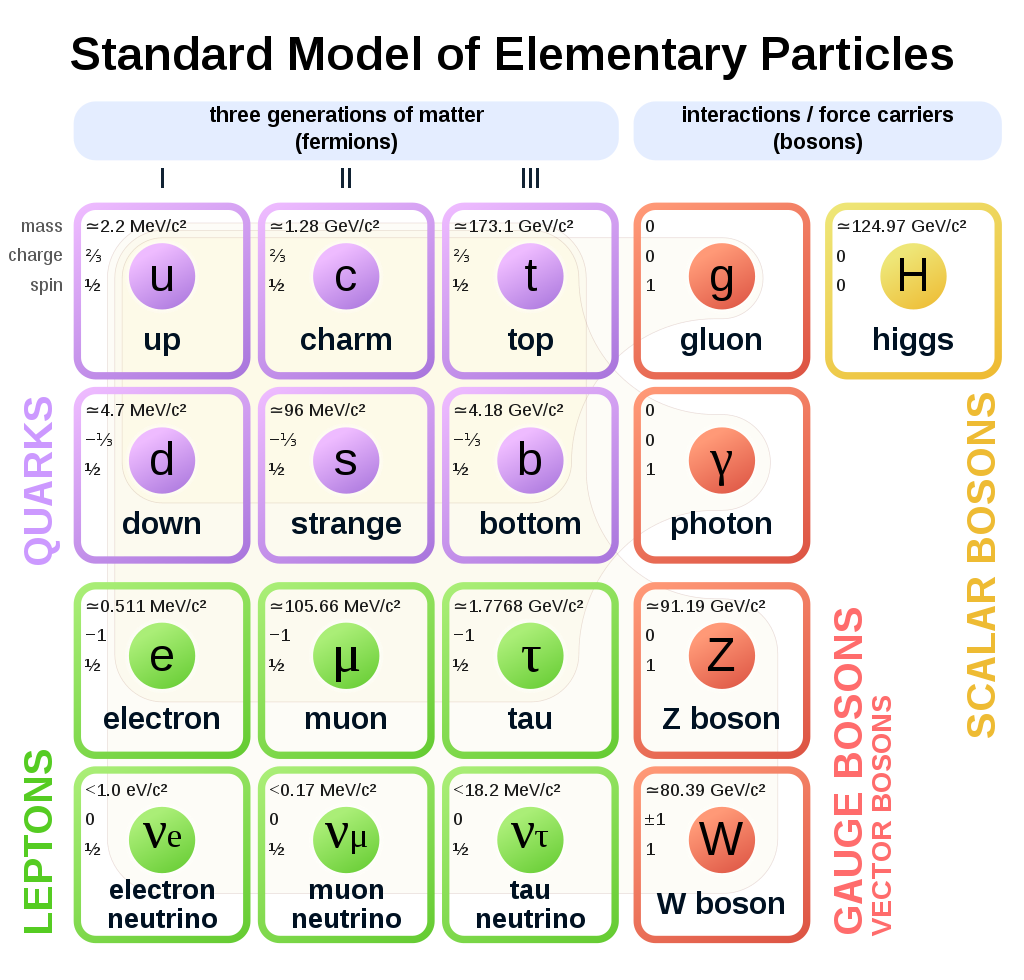
\includegraphics[width=0.85\linewidth]{standardmodel}
	\caption{Overview of all the ingredients of the Standard Model which constitutes all the fermions and the gauge bosons. Elementary properties like mass, electric charge and spin of all the particles are also shown in the image.~\cite{standardmodelpicture}}
	\label{fig:theory:standardmodel}
\end{figure}



%------------------------------------------------------------------------------
\subsection{Gauge groups}%
\label{sec:theory:standardmodel:gauge}
%------------------------------------------------------------------------------
The Standard Model is formed from the combination of three different local symmetry groups which can be written as~\cite{halzen}:
\begin{equation}
\text{SU(3)}_{\text{c}} \times \text{SU(2)}_{\text{L}} \times \text{U(1)}_{\text{Y}} \,,
\end{equation}
where SU(3)$_{\text{c}}$ symmetry group is generated by the colour charge associated with the strong interaction, described in section \ref{sec:theory:standardmodel:strong}. The SU(2)$_{\text{L}} \times$ U(1)$_{\text{Y}}$ symmetry groups represent the left-handed isospin and hypercharge symmetries within the SM, which are generated by the unified electroweak interaction, described in section \ref{sec:theory:standardmodel:weak}. 

These local symmetries are applied to the SM Lagrangian ($\mathcal{L}_{\text{SM}}$) which correspond to local gauge invariance. The SM Lagrangian can be written as~\cite{halzen}:

\begin{equation}
\mathcal{L}_{\text{SM}} = \mathcal{L}_{\text{Boson}} + \mathcal{L}_{\text{Fermion}} + \mathcal{L}_{\text{Yukawa}} + \mathcal{L}_{\text{Higgs}} \,,
\end{equation}
where $\mathcal{L}_{\text{Boson}}$ + $\mathcal{L}_{\text{Fermion}}$ represents the kinetic energies, electroweak interaction and self-interaction of fermions and bosons. $\mathcal{L}_{\text{Yukawa}}$ is a term from Yukawa coupling which gives mass to the particles. $\mathcal{L}_{\text{Higgs}}$ describes the spontaneous symmetry breaking by Higgs field.

%------------------------------------------------------------------------------
\subsection{Particle interaction}%
\label{sec:theory:standardmodel:interaction}
%------------------------------------------------------------------------------

%------------------------------------------------------------------------------
\subsubsection{Electromagnetic interaction}%
\label{sec:theory:standardmodel:em}
%------------------------------------------------------------------------------
The electromagnetic interaction (EM) is described by one of the Quantum Field Theory (QFT), known as Quantum electrodynamics (QED). It is based on the $\text{U(1)}_{\text{Y}}$ gauge group which represents the interaction between the charged fermions and a massless gauge boson known as a photon. Photon (\Pphoton) is a vector gauge boson which acts as a force carrier of the EM interaction. Only neutrinos (and their antiparticles) do not interact via the EM interaction because they are electrically neutral. $\text{U(1)}_{\text{Y}}$ is abelian in nature which means it is a commuting gauge group that does not allow any self-interaction terms for the photon field.

The QED Lagrangian for a charged fermion ($\psi$) of mass $m$ can be written as:
\begin{equation}
\mathcal{L}_{\text{QED}} = \bar{\psi} \, (i\textbf{D}_{\text{QED}} - m) \, \psi - \frac{1}{4}F_{\mu\nu}F^{\mu\nu} \,,
\end{equation}
where $F$ is the electric field tensor which can be expressed in terms of the photon vector field by $F^{\mu\nu} = \partial^{\mu}A^{\nu} - \partial^{\nu}A^{\mu}$ and $\textbf{D}_{\text{QED}}$ is a covariant derivative which also depends on the photon vector field $A$.~\cite{halzen}

%------------------------------------------------------------------------------
\subsubsection{Strong interaction}%
\label{sec:theory:standardmodel:strong}
%------------------------------------------------------------------------------
The strong interaction is described by a theory called the Quantum Chromodynamics (QCD). It explains the interaction between partons which include quarks and gluons. Gluons (\Pgluon) are vector gauge boson which mediates the strong interaction. Like electric charge in the QED, QCD also introduces a new type of property called colour charge. There are three different types of colour charges: red, blue and green. So, all the six types of quarks and their antiparticles can be represented as colour triplets. Particles carrying a colour charge can feel the effects of the strong interaction. The strong force is described by the $\text{SU(3)}_{\text{c}}$, which is a non-abelian gauge group that means it allows the self-interaction terms for the gluons. Due to the non-abelian nature of the force, it is more complex than the EM force, and give rise to eight different coloured gluons.~\cite{halzen}

The strong interaction is the strongest among all the three interactions described in the SM. One of the consequences of the QCD is the process of hadronisation which means that partons can only exist in bound colour neutral states called hadrons, such as the proton. The strength of the coupling constant of the strong interaction increases with the distance between the coloured particles due to the gluon self-interaction. If one tries to separate the two quarks within a hadron, a large amount of energy is required, and at some point it spontaneously produces a quark-antiquark pair, turning the initial hadron into a pair of hadrons instead of producing an isolated coloured quark. This phenomenon is known as \textit{colour confinement}. The process in which the hadrons are formed from the partons is called hadronisation. It cannot be described using standard perturbation theory since it takes place in the non-perturbative regime of the QCD where the strong coupling is larger than one. The strength of the coupling constant of the strong interaction is low at small distances, so the quarks can exist freely inside the hadrons. This feature of the QCD is known as \textit{asymptotic freedom}.~\cite{thomson}

There are two groups of hadrons: baryons and mesons. Baryons are made up of three quarks or antiquarks while mesons are made from a quark-antiquark pair. The effects of the hadronisation can be seen as clusters in the particle detectors, which are further reconstructed as jets. Jets are the important physics object for this thesis and are discussed in detail in Chapter \ref{sec:jetsandtaggers}.

The QCD Lagrangian for a coloured charged fermion ($\psi$) of mass $m$ can be written as:
\begin{equation}
\mathcal{L}_{\text{QCD}} = \bar{\psi}_{j} \, (i\gamma^{\mu}\textbf{D}_{\text{QCD,}\,\mu} - m_{j}) \, \psi_{j} - \frac{1}{4}G_{\mu\nu}^{\alpha}G^{\mu\nu}_{\alpha} \,,
\end{equation}
where $G_{\mu\nu}^{\alpha}$ is a gluon field tensor which includes the additional self-interaction term of the gluon vector fields and $\alpha$ is denoted as the eight coloured gluons. $\textbf{D}_{\text{QCD,}\mu}$ is a covariant derivative which can be expressed in terms of the gluon gauge field $A_{\mu}^{\alpha}$ and the strong coupling constant $\alpha_{\text{s}}$. Index $j$ is indicated as all the coloured flavours of the quarks.~\cite{halzen}

%------------------------------------------------------------------------------
\subsubsection{Weak interaction and Electroweak unification}%
\label{sec:theory:standardmodel:weak}
%------------------------------------------------------------------------------
The weak interaction is described by a theory called the Quantum Flavourdynamics (QFD). It explains the interaction between particles that is responsible for the radioactive decay of atoms. The Lagrangian of the weak interaction is constructed only from left-handed doublets in the $\text{SU(2)}_{\text{L}}$ gauge group since right-handed particles in the SM appeared as singlets and are not affected by the weak force. The weak force is better understood in terms of the Electroweak theory (EWT).~\cite{halzen}


In the Standard Model, the electromagnetic and weak interactions are unified at an energy of electroweak scale and described by the EWT proposed by Glashow, Salam and Weinberg. The electroweak interaction is described by $\text{SU(2)}_{\text{L}} \times \text{U(1)}_{\text{Y}}$ gauge group where L denotes the SU(2) doublet and singlet representation of left-handed particles and Y is denoted as the weak hypercharge, given as $\text{Y}=q-T_{3}$. Here, $T_{3}$ is the third component of the weak isospin and $q$ is electric charge.~\cite{halzen}

The electroweak Lagrangian for fermions can be written as:
\begin{equation}
\mathcal{L}_{\text{EW}} = \bar{\psi}_{f} \, (i\gamma^{\mu}\textbf{D}_{\text{EW,}\,\mu}) \, \psi_{f} \,,
\end{equation}
where the fermionic fields $\psi_{f}$ are organised in $\text{SU(2)}_{\text{L}}$ doublets and singlet, as shown below:

\begin{equation}
\psi_{\text{lepton}} = \begin{pmatrix} \Pnue \\ e \end{pmatrix}_{L}, \begin{pmatrix} \Pnum \\ \mu \end{pmatrix}_{L}, \begin{pmatrix} \Pnut \\ \tau \end{pmatrix}_{L}, e_{R}, \mu_{R}, \tau_{R} \,,
\end{equation}

\begin{equation}
\psi_{\text{quark}} = \begin{pmatrix} u \\ d \end{pmatrix}_{L}, \begin{pmatrix} c \\ s \end{pmatrix}_{L}, \begin{pmatrix} t \\ b \end{pmatrix}_{L}, u_{R}, d_{R}, c_{R}, s_{R}, t_{R}, b_{R} \,.
\end{equation}
The EWT is a parity-violating theory, so right-handed neutrinos are omitted in the SM. There are four vector fields which contribute to the electroweak interaction. A linear combination of $W^{1}_{\mu}$ and $W^{2}_{\mu}$ describes the two charged $W$ bosons, as shown below:
\begin{equation}
W^{\pm}_{\mu} = \frac{1}{\sqrt{2}}(W^{1}_{\mu} \mp iW^{2}_{\mu}) \,.
\end{equation}
And the linear combination of $W^{3}_{\mu}$ and $B_{\mu}$ represents the two neutral bosons, the $Z$ boson and the photon as shown below:
\begin{align}
A_{\mu} = \sin\theta_{W}W^{3}_{\mu} + \cos\theta_{W}B_{\mu} \,, \\
Z_{\mu} = \cos\theta_{W}W^{3}_{\mu} - \sin\theta_{W}B_{\mu} \,,
\end{align}
where $\theta_{W}$ is called the Weinberg angle and is given by $\tan\theta_{W} = \frac{g}{g'} \,,$ and $g$ and $g'$ are the gauge coupling constants.~\cite{halzen}

%------------------------------------------------------------------------------
\subsection{Higgs mechanism}%
\label{sec:theory:standardmodel:higgs}
%------------------------------------------------------------------------------
The addition of mass term to the Lagrangian shown before breaks the gauge symmetry of the model, so a different process is required for particles to become massive. The process which describes how particles acquire their mass, without breaking the gauge invariance of the SM, is called the Higgs mechanism. The Higgs mechanism introduces \textit{spontaneous symmetry breaking} of the $\text{SU(2)}_{\text{L}} \times \text{U(1)}_{\text{Y}}$ gauge group by adding a new complex scalar doublet field, called the Higgs field.~\cite{halzen} 

Let us consider a weak isospin doublet of two complex fields ($\Phi$):
\begin{equation}
\Phi = \begin{pmatrix} \phi^{+} \\ \phi^{o} \end{pmatrix} \,.
\end{equation}
Then the potential $\mathcal{U}(\Phi)$ given by the complex field can be written as:
\begin{equation}
\mathcal{U}(\Phi) = \mu^{2}(\Phi^{*}\Phi) + \lambda(\Phi^{*}\Phi)^{2} \,.
\end{equation}
Only solution with $\lambda>0$ and $\mu^{2}<0$ is considered so that the energy of the potential is bounded below and leads to a non-unique ground state energy. The minimum of this potential is not at the zero value of the field and is given by $v = \sqrt{\mu^{2}/\lambda}$. Now the Lagrangian can be written as~\cite{halzen}:
\begin{equation}
\mathcal{L}_{Higgs} = |\textbf{D}_{\mu}\Phi|^{2} - \mu^{2}(\Phi^{*}\Phi) - \lambda(\Phi^{*}\Phi)^{2} \,.
\end{equation}
By expanding the Lagrangian around the vacuum expectation value ($vev$), a mass term is introduced for the vector bosons. The masses of the bosons predicted by this mechanism are related in the following way:

\begin{align}
m_{\text{W}^{\pm}} = \frac{1}{2}vg \,, \\
m_{\text{Z}} = \frac{1}{2}v\sqrt{g^{2} + g'^{2}} \,, \\
\cos\theta_{W} = \frac{m_{\text{W}}}{m_{\text{Z}}} \,, \\
m_{\text{H}} = \sqrt{2}\mu \,.
\end{align}
The Higgs mechanism
proposes the existence of the Higgs boson ($H$) with $m_{\text{H}}=\SI{125}{\giga\electronvolt}$ which was confirmed in 2012 by the ATLAS and CMS collaborations at CERN.~\cite{higgsatlas}~\cite{higgscms} Fermions also acquire masses through the Higgs mechanism by interactions between the fermionic and Higgs scalar fields, called Yukawa couplings.~\cite{halzen}

%------------------------------------------------------------------------------
\subsection{Feynman diagram}%
\label{sec:theory:standardmodel:feynmandiagram}\index{feynmandiagram}
%------------------------------------------------------------------------------
A Feynman diagram is a graphical representation of the particle interaction. For calculating the probability of the particle interaction to happen, the scattering matrix has to be evaluated. By satisfying the conservation laws of energy and momentum, the scattering matrix ends up with the invariant Matrix Element |$\mathcal{M}$|. A Feynman diagram is a technique which is used to evaluate |$\mathcal{M}$|. It consists of different components which are associated with some mathematical expressions that are defined by Feynman rules.~\cite{thesis:rui}

A Feynman diagram consists of a point, called vertex, and lines attached to the vertex. A vertex represents the interaction of particles, which could either be the emission or absorption of a particle or the flavour change of a particle. There are three different types of lines: internal lines which connect two vertices, also known as a propagator, and the two types of external lines in which first the incoming lines that extend to a vertex representing an initial state and the second when the outgoing lines extend from a vertex representing the final state of the process. The external lines denote the real visible particles (or antiparticles), whereas internal lines denote virtual particles. The main difference between the two types of particles is that virtual particles do not obey the energy-momentum relation, whereas the real particles obey. 

Each vertex represents a point of interaction which could either be one of the three interactions. The strength of the interaction is given by the coupling constant $g$, which is shown for all the three interactions below:

\[\text{EM: }g = qe \,, \hspace{2cm} \text{Weak: }g = g_{\text{W}} \,, \hspace{2cm} \text{Strong: }g = \sqrt{\alpha_{\text{s}}} \,, \]
where $q$ is denoted as the electric charge, $g_{\text{W}}$ is represented as the coupling constant of the weak interaction and $\alpha_{\text{s}}$ is denoted as dimensionless strong interaction coupling constant. At each vertex, the conservation of energy, momentum, angular momentum, charge, lepton number and baryon number should be followed.


%------------------------------------------------------------------------------
\subsection{Drawbacks of the Standard Model}%
\label{sec:theory:standardmodel:drawbacks}\index{drawbacks}
%------------------------------------------------------------------------------
The Standard Model is the most rigorous theory of particle physics. It is incredibly precise and accurate in its predictions. It gives a reliable predictive model of the particles and their interactions. However, it cannot explain several phenomena. In order to solve this, several theories have been proposed. Unfortunately, there has been no experimental evidence of these theories yet. Some of the phenomena are discussed in detail below:

\begin{itemize}
\item \textbf{Hierarchy problem:} all the particles in the SM gain their masses by their interaction with the Higgs boson. However, the radiative corrections to the mass of the Higgs boson conflict with the experimental value of Higgs mass. These corrections diverge quadratically  up to the cut-off scale of new physics $\Lambda$, where the SM is no longer valid.

The radiative corrections appear in virtual loop diagrams of particles that couple to the Higgs field. This means that a considerable amount of \enquote{fine-tuning} is required to keep the Higgs mass at the electroweak scale ($\approx\SI{100}{\giga\electronvolt}$) if the SM is to remain valid up to high energies. The unnatural amount of fine-tuning to the Higgs mass is known as the \textit{hierarchy problem}. The radiative corrections to the Higgs mass can be expressed as:

\begin{equation}
	\Delta m_{H}^{2} = -\frac{\lambda^{2}_{f}}{8\pi^{2}} \left[\Lambda^{2} + ... \right] \,,
\end{equation}
where $\lambda_{f}$ is the Yukawa coupling of any fermion. The Hierarchy problem implies that there should be new physics at the \si{\tera\electronvolt} scale that eliminates the large loop contributions. Some of the possibilities for this to happen are supersymmetery (SUSY)~\cite{hierarchy2}, Gauge-Higgs unification~\cite{gaugehiggs}, composite Higgs~\cite{hierarchy2}, extra dimensions~\cite{extradim}, etc.

\item \textbf{Neutrino masses:} the Standard Model predicts that neutrinos should be massless like photons. However, experiments with solar, atmospheric, and accelerator neutrinos have provided compelling evidence that the three neutrinos oscillate between their flavours as they move. This is only possible if the neutrinos have some mass. These neutrino masses are quite small ($<\SI{0.1}{\electronvolt}$). Some experimental results have also suggested that there might be a fourth type of neutrino called the sterile neutrinos which are still yet to discover \cite{neutrinomass}.

\item \textbf{Matter-antimatter asymmetry:} whenever matter is created, usually its counterpart antimatter is also formed. It is believed that at the time of the Big Bang, matter and antimatter were produced in equal parts. But what we see today is that matter is dominant. This behaviour is unexplained by the SM. To achieve this asymmetry, theories should have to violate the CP (charge-parity), baryon number and lepton number conservation laws.

\item \textbf{Dark matter and dark energy:} In the universe, galaxies usually rotate with high speed, which means that the gravitational force generated by their matter should not be able to balance the centripetal force. But what we observe is that it holds them together, which means that there should be an extra force generated by some additional matter. This unknown matter is called dark matter.~\cite{darkmatter} It is believed that dark matter constitutes roughly 27\% of the universe, whereas dark energy represents 68\% of the universe, leaving about 5\% of the matter. However, the SM can only explain this tiny fraction of matter which we can see.

\item \textbf{Gravity:} the SM could not be able to explain the fourth type of fundamental force known as the gravitational force. It does not seem to have any impact on the subatomic interactions. But some theories state that there is an existence of a subatomic particle called graviton, which might transmit the gravitational force the same way as photons mediate the electromagnetic force.~\cite{drawbacks}

\item \textbf{Free parameters:} the SM has 19 free parameters whose values are experimentally determined, but there is no theoretical prediction of these values. This gives us a strong indication to extend our knowledge of the Standard Model to explain these results \cite{thesis:anji}.
\end{itemize}

\clearpage
%------------------------------------------------------------------------------
\section{Vector-like quarks (VLQs)}%
\label{sec:theory:vectorlikequarks}
%------------------------------------------------------------------------------

With the discovery of the Higgs boson, the Standard Model is the most comprehensive theory which can explain all the known elementary particles and their interactions. However, there are some shortcomings to this theory which are discussed in the last section. There are some theories which were formulated by considering the principles which are beyond the scope of the SM, called Beyond Standard Model (BSM) theories. These theories are based on several models which predict the existence of new particles that can cancel the divergence of the radiative corrections to the Higgs mass and solve the Higgs mass hierarchy problem. These new particles include the fourth-generation quarks, called vector-like quarks.

Vector-like quarks (VLQs) are hypothetical spin $\frac{1}{2}$ coloured particles. The chiral fourth-generation quarks (\Ptop' and \Pbottom'), which have identical features like the SM third-generation quarks (\Ptop and \Pbottom), are eliminated because their existence impact a significant effect on the production cross-section of the Higgs. But, VLQs on the otherhand show a much smaller impact on the production cross-section of the Higgs, which are even comparable to the uncertainty of the current measurements. Several models of new physics, such as Little Higgs models~\cite{little_higgs}, or those predicting the composite Higgs boson~\cite{composite_higgs}, also include VLQs. They do not receive their mass by the Higgs boson Yukawa coupling. Many models also assume their mixing with the SM third-generation quarks because of the large masses of \Ptop- and \Pbottom-quark.~\cite{vlqpaper}

SM quarks are chiral in nature because their left-handed and right-handed components transform differently under $\text{SU(2)}_{\text{L}} \times \text{U(1)}_{\text{Y}}$ gauge groups, whereas for VLQs, both the components transform similarly. The Lagrangian of the charged current can be written as:
\begin{equation}
	\mathcal{L}_{W} = \frac{g}{\sqrt{2}}(J^{\mu+}W_{\mu}^{+} + J^{\mu-}W_{\mu}^{-}) \,,
\end{equation}
where $J^{\mu\pm} = J^{\mu\pm}_{L} + J^{\mu\pm}_{R}$ and is known as the current density.

SM quarks only have contributions from the left-handed component, which is a mixture of both vector and axial-vector quantities, known as V-A interaction. Whereas in the case of VLQs, both left- and right-handed components have a contribution which together cancels out the axial-vector term and results in the vector quantity and therefore called vector-like quarks.~\cite{vlqinteraction}



%------------------------------------------------------------------------------
\subsection{Multiplet representation}%
\label{sec:theory:multipletrepresentation}
%------------------------------------------------------------------------------

There are four types of vector-like quarks which are listed below along with their electric charges:
\[T  = +\frac{2}{3} \,, B = -\frac{1}{3} \,, \]
\[X  = +\frac{5}{3} \,, Y = -\frac{4}{3} \,. \]
They are represented by different multiplet models, which depend on their weak isospin states. Table \ref{table:theory:multipletrepresentation} shows the different multiplet models and the VLQ candidates along with their weak isospin and the hypercharge. $T$ quark can belong to any multiplet, while $Y$ quark can only exist under doublet and triplet models.



\begin{table}[hbt!]
	\centering
	\begin{tabular}{c | c | c | c} 
		\toprule
		& Singlet & Doublet & Triplet \\
		\midrule
		$Q_{q}$ & 
		$T_{\text{$+\frac{2}{3}$}}$ \hspace{0.4cm} $B_{\text{$-\frac{1}{3}$}}$ & 
		$\begin{pmatrix} X_{\text{$+\frac{5}{3}$}} \\ T_{\text{$+\frac{2}{3}$}} \\ \end{pmatrix}$ \hspace{0.4cm}
		$\begin{pmatrix} T_{\text{$+\frac{2}{3}$}} \\ B_{\text{$-\frac{1}{3}$}} \\ \end{pmatrix}$ \hspace{0.4cm}  
		$\begin{pmatrix} B_{\text{$-\frac{1}{3}$}} \\ Y_{\text{$-\frac{4}{3}$}} \\ \end{pmatrix}$ & 
		$\begin{pmatrix} X_{\text{$+\frac{5}{3}$}} \\ T_{\text{$+\frac{2}{3}$}} \\ B_{\text{$-\frac{1}{3}$}} \\ \end{pmatrix}$ \hspace{0.4cm} 
		$\begin{pmatrix} T_{\text{$+\frac{2}{3}$}} \\ B_{\text{$-\frac{1}{3}$}} \\ Y_{\text{$-\frac{4}{3}$}} \\ \end{pmatrix}$ \\ 
		\midrule
		
		$T_{\text{3}}$ & 0 \hspace{0.6cm} 0 & $\frac{1}{2}$ \hspace{1.1cm} $\frac{1}{2}$ \hspace{1.1cm} $\frac{1}{2}$ & 1 \hspace{1.1cm} 1 \\ 

		$Y$ & $+\frac{4}{3}$ \hspace{0.4cm} $-\frac{2}{3}$ & $+\frac{7}{3}$ \hspace{0.9cm} $-\frac{1}{3}$ \hspace{0.9cm} $+\frac{5}{3}$ & $+\frac{4}{3}$ \hspace{0.9cm} $-\frac{2}{3}$ \\ 
		\bottomrule
	\end{tabular}
	\caption{Overview of the different multiplet models of VLQs along with their isospin $T_{\text{3}}$, hypercharge $Y$ and electric charge $q$.}
	\label{table:theory:multipletrepresentation}
\end{table}


This thesis focuses on the production of $T$ or $Y$ quark decaying into $Wb$, for which the interesting candidates are $T$ quark from ($T$) singlet, $Y$ quark from ($B, Y$) doublet and only $Y$ quark from ($T, B, Y$) triplet. $T$ quark from ($T, B, Y$) triplet does not couple to $Wb$. $T$ quark can decay into either $Wb$, $Zt$ or $Ht$ but at the high mass limit, the branching ratio converges to 2:1:1 ($Wb: Zt: Ht$). On the other hand, $Y$ quark can only decay into $Wb$ because of its charge and therefore, $\mathcal{B}(Y \rightarrow Wb) = 100\%$. That implies that $T$ quark can be produced by the fusion of either $Wb$, $Zt$ or $Ht$ but $Y$ quark can only be produced by the fusion of $W$ boson and $b$-quark.


%------------------------------------------------------------------------------
\subsection{Production of VLQs}%
\label{sec:theory:production}
%------------------------------------------------------------------------------

VLQs can either be can be produced via single and pair production in proton-proton ($pp$) collisions at the LHC. 

\begin{figure}[hbt!]
	\centering
	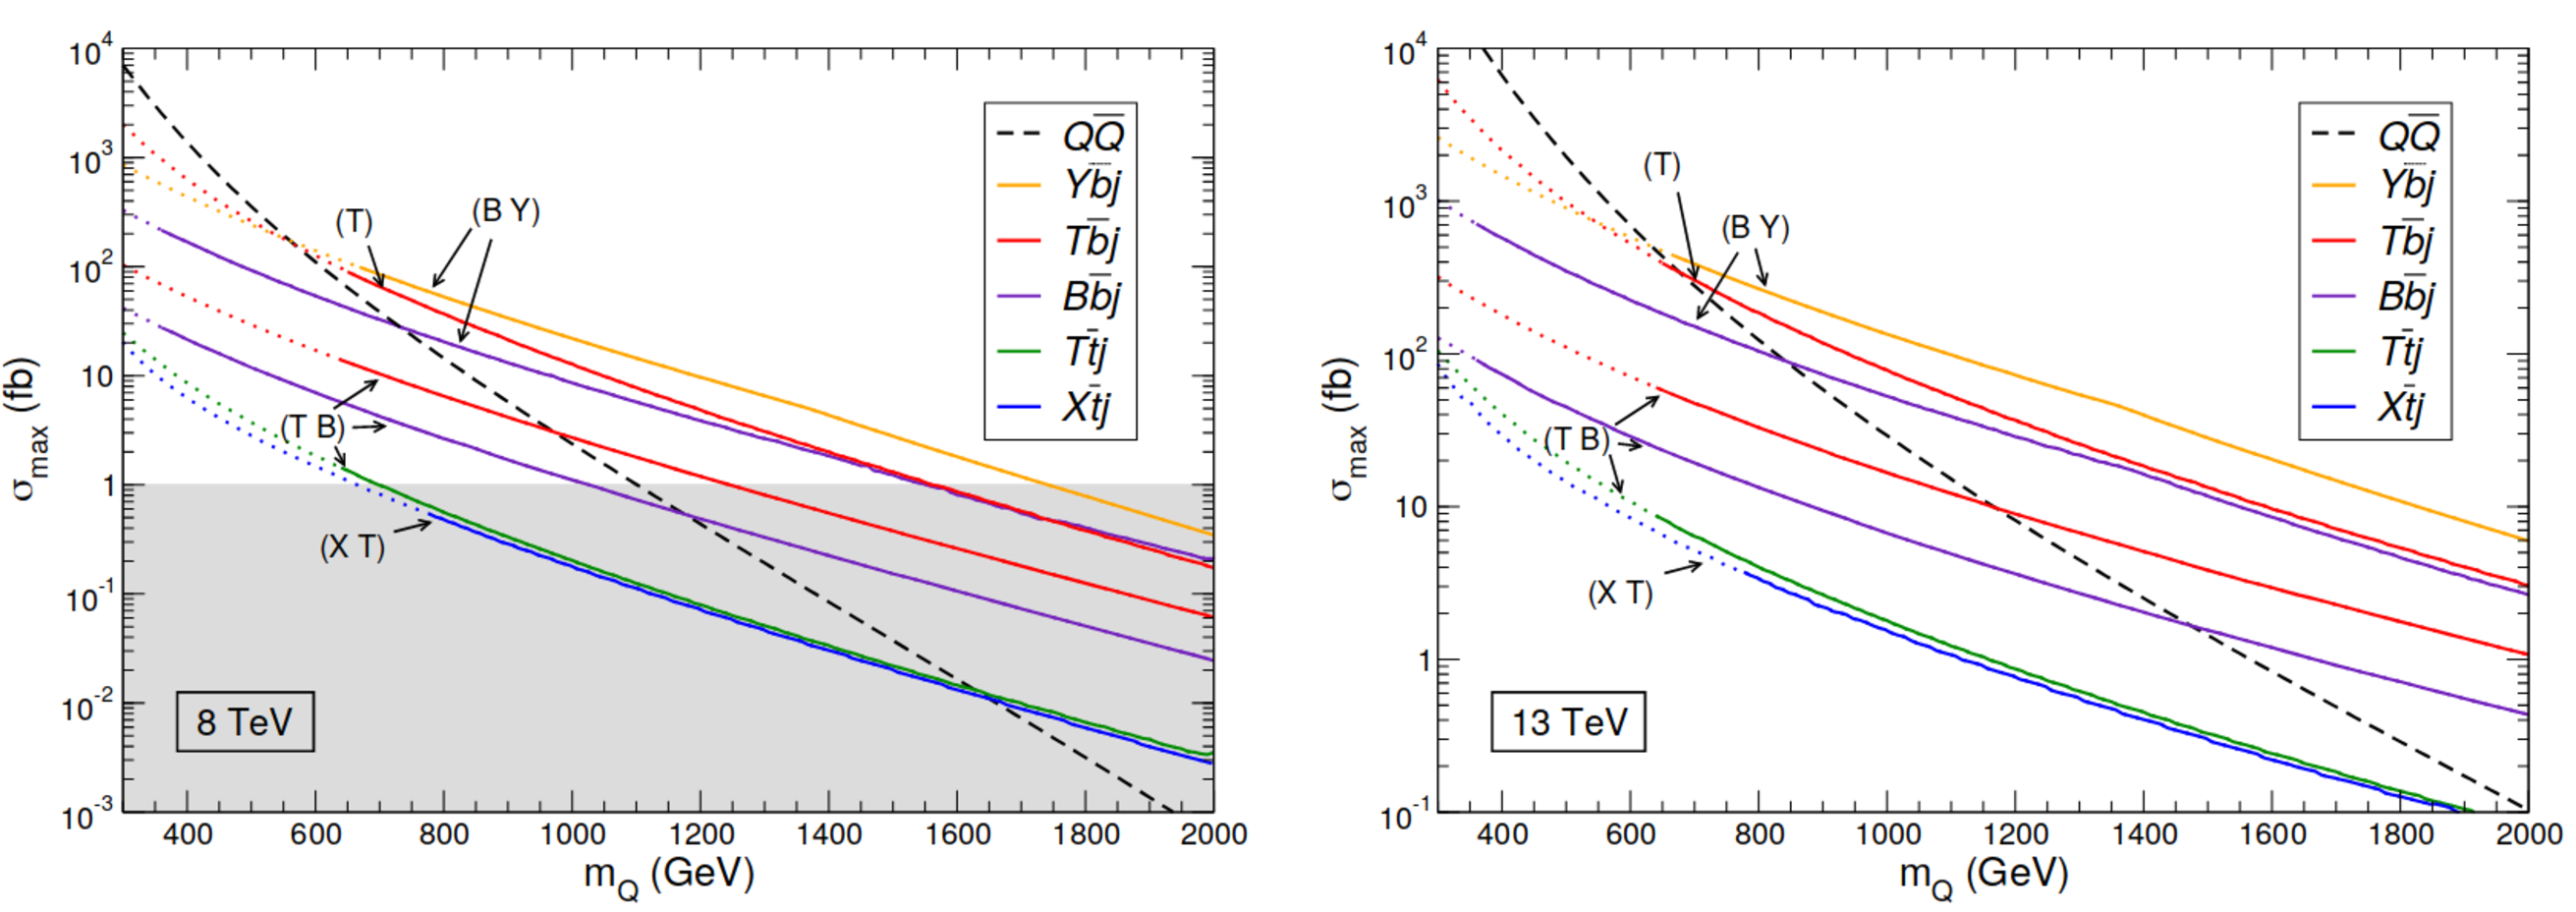
\includegraphics[width=\linewidth]{production.pdf}
	\caption{Production cross-section for single VLQ production and VLQ pair production as a function of VLQ mass at $\sqrt{s}=\SI{8}{\tera\electronvolt}$ and $\sqrt{s}=\SI{13}{\tera\electronvolt}$. The pair production process is denoted by dotted line whereas coloured lines show different single VLQ processes. Both the plots show that single production processes have larger production cross-section at high VLQ mass.~\cite{aguilar}}
	\label{fig:theory:production}
\end{figure}

\begin{itemize}
\item \textbf{Single VLQ production:} VLQs can be produced by the fusion of the SM gauge boson and third-generation quark, which is enabled by their strong coupling to the SM quarks. Therefore, searches for singly produced VLQs can be used to probe these couplings as a function of the VLQ mass. Single VLQ production is a dominant process at high VLQ masses in both $\sqrt{s}=\SI[per-mode=symbol]{8}{\tera\electronvolt}$ and $\sqrt{s}=\SI[per-mode=symbol]{13}{\tera\electronvolt}$, which can be seen from Fig.\ \ref{fig:theory:production}. The Feynman diagram for two possible single VLQ production processes is shown in Fig \ref{fig:theory:production:single}. In this thesis, the focus is the single production process of $T$ or $Y$ quark, as shown in Fig.\ \ref{fig:theory:production:single:ty}.

\begin{figure}[hbt!]
	\centering
	\begin{subfigure}{.4\textwidth}
		\centering
		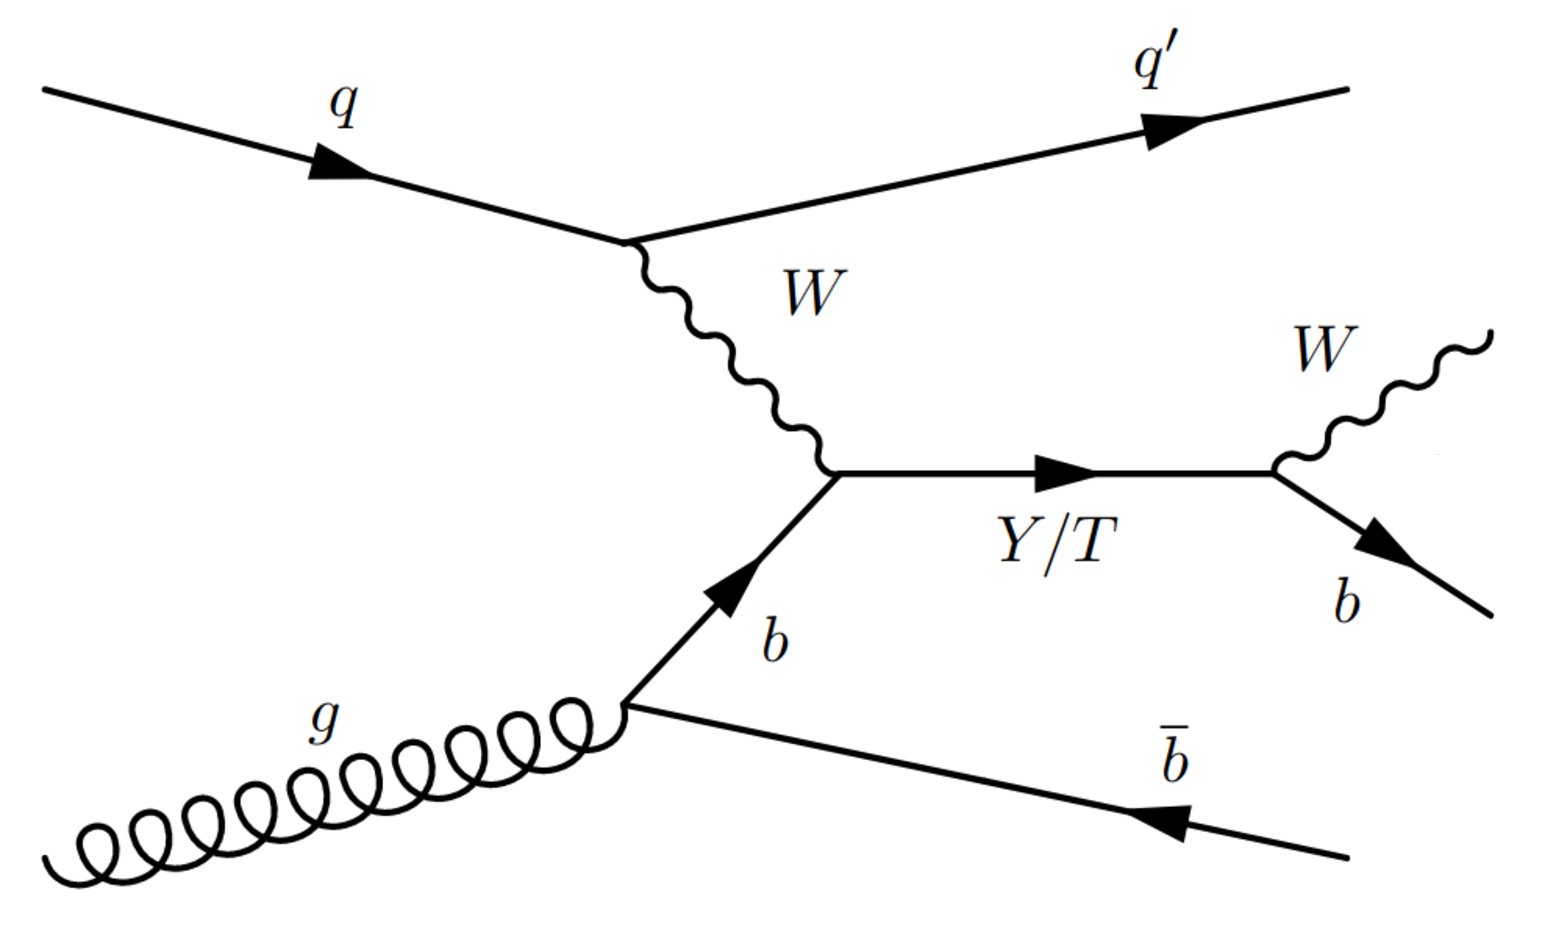
\includegraphics[width=\linewidth,height=\textheight,keepaspectratio]{singleproduction1.pdf}
		\caption{}
		\label{fig:theory:production:single:ty}
	\end{subfigure}\hspace{1cm}
	\begin{subfigure}{.35\textwidth}
		\centering
		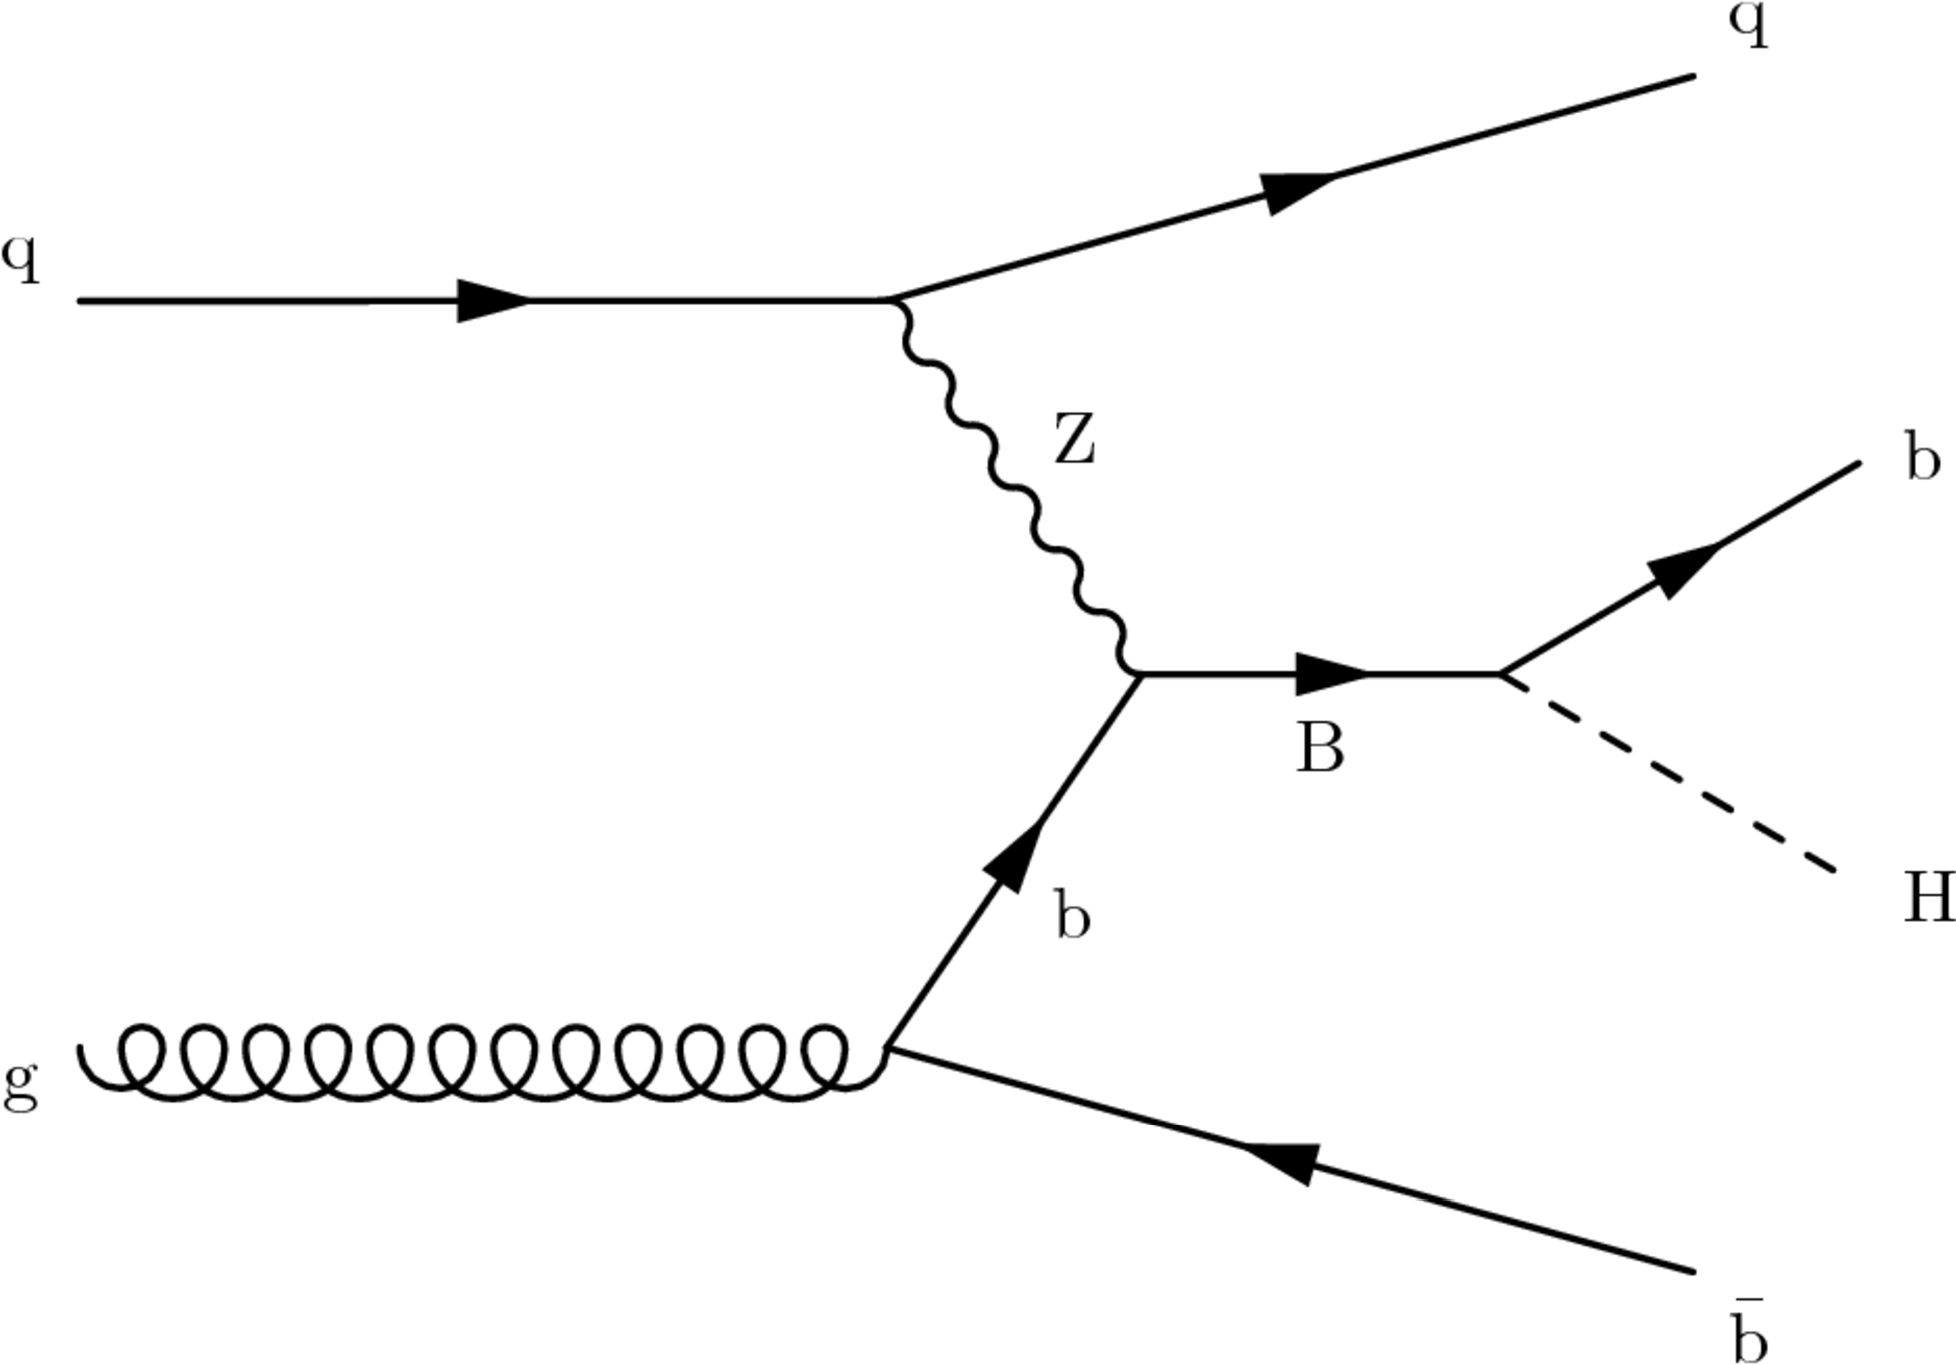
\includegraphics[width=\linewidth,height=\textheight,keepaspectratio]{singleproduction2.pdf}
		\caption{}
		\label{fig:theory:production:single:b}
	\end{subfigure}
	\caption{Feynman diagrams for single VLQ production, where (a) shows the production of $T/Y$ quark by the fusion of $W$ and $b$-quark and (b) shows the production of $B$ quark by the fusion of $Z$ and $b$-quark.~\cite{vlqpaper}}
	\label{fig:theory:production:single}
\end{figure}

\item \textbf{VLQ pair production:} VLQs can be produced in pair which allows to set a limit on VLQ masses. These masses are insensitive to the coupling because they are produced through the strong interaction. Pair production is a dominant process at lower VLQ masses in both  $\sqrt{s}=\SI[per-mode=symbol]{8}{\tera\electronvolt}$ and $\sqrt{s}=\SI[per-mode=symbol]{13}{\tera\electronvolt}$, which can be seen from Fig. \ref{fig:theory:production}. The Feynman diagram for a pair production process is shown in Fig.\ \ref{fig:theory:production:pair}.

\begin{figure}[hbt!]
	\centering
	\begin{subfigure}{.4\textwidth}
		\centering
		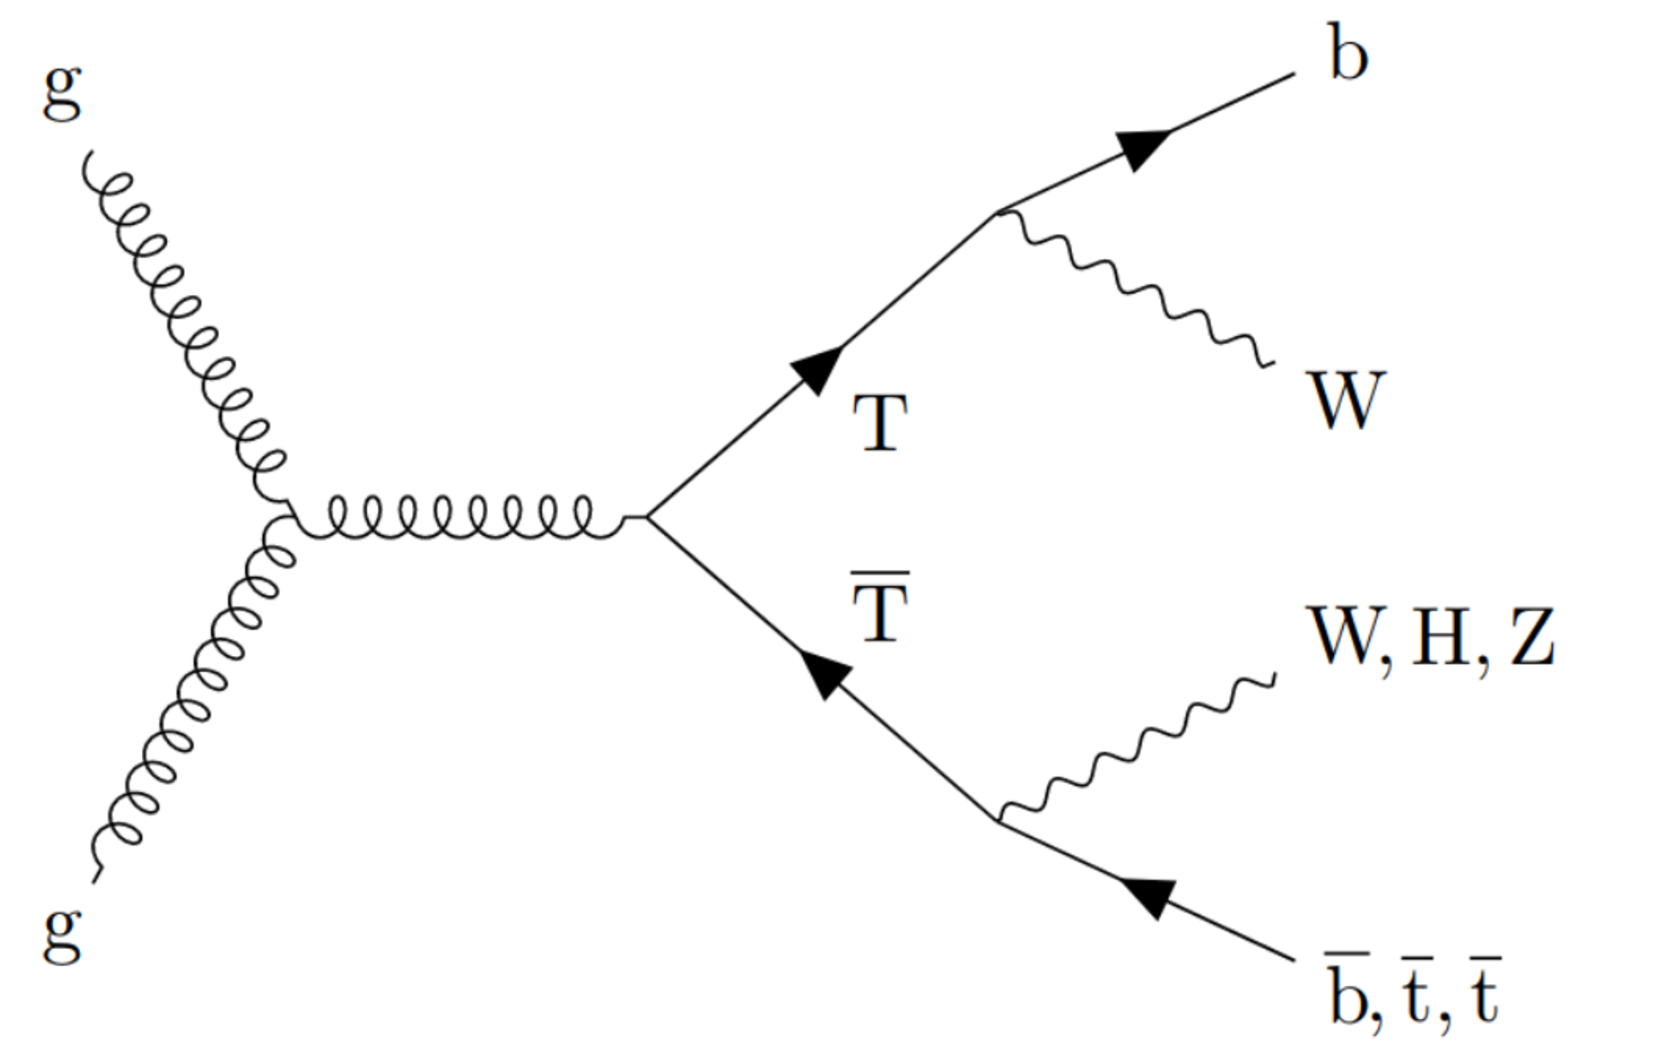
\includegraphics[width=\linewidth,height=\textheight,keepaspectratio]{pairproduction1.pdf}
		\caption{}
		\label{fig:theory:production:pair:t}
	\end{subfigure}
	\caption{Feynman diagram for VLQ pair production where $T\bar{T}$ is produced in pair, which can further decay into $Wb$, $Ht$ or $Zt$ pair.~\cite{pairproductiont}}
	\label{fig:theory:production:pair}
\end{figure}

\end{itemize}


%------------------------------------------------------------------------------
\subsection{Models}%
\label{sec:theory:models}
%------------------------------------------------------------------------------

Several theories have been proposed for describing the characteristics of VLQs. In this thesis, two different models have been presented that use different formulations of the Lagrangian. The Lagrangian depends on the different parameterisation that explains these new particles and their interactions. 

\begin{itemize}
\item \textbf{Renormalisable theory:} 
In this model, the Lagrangian is parameterised by a mixing angle $\theta_{\text{L,R}}$, which describes the mixing between the SM quarks and VLQs. This theory gives a complete information about the dependence of branching ratios on the multiplet dimensions. Hence, a given value of either left- or right-handed mixing angle $\theta_{\text{L}}$ or $\theta_{\text{R}}$ entirely determines all the branching ratios of VLQ at any mass point.~\cite{aguilar}

\item \textbf{General theory:} According to this theory, the Lagrangian is parameterised by a non-renormalisable coupling term $c_{\text{L,R}}^{\text{Wb}}$. This theory can predict the production cross-section of VLQs at next-to-leading-order terms (NLO).~\cite{wulzer}
\end{itemize}

By comparing the respective Lagrangians of the renormalisable model and general model, a relation is established between the coupling terms $c_{\text{L,R}}^{\text{Wb}}$ and the mixing angles $\theta_{\text{L,R}}$ within a given multiplet and is shown by the equations below:

\begin{equation}
c_{\text{L,R}}^{\text{Wb}} = \sqrt{2}\sin\theta_{\text{L,R}} \,,
\label{eqn:theory:models:singlet}
\end{equation}

\begin{equation}
c_{\text{L}}^{\text{Wb}} = 2\sin\theta_{\text{L}} \,,
\label{eqn:theory:models:triplet}
\end{equation}
where Eqn.\ \ref{eqn:theory:models:singlet} is true for $T$ singlet and ($B,Y$) doublet model, and Eqn.\ \ref{eqn:theory:models:triplet} is valid for ($T,B,Y$) triplet model. These relations are only valid within the renormalisable formulation, and if one considers only the interaction between $T/Y$, \PW and \Pbottom.~\cite{vlqpaper}



%%% Local Variables: 
%%% mode: latex
%%% TeX-master: "mythesis"
%%% End: 
